% Options for packages loaded elsewhere
\PassOptionsToPackage{unicode}{hyperref}
\PassOptionsToPackage{hyphens}{url}
\PassOptionsToPackage{dvipsnames,svgnames,x11names}{xcolor}
%
\documentclass[
  letterpaper,
  DIV=11,
  numbers=noendperiod]{scrartcl}

\usepackage{amsmath,amssymb}
\usepackage{iftex}
\ifPDFTeX
  \usepackage[T1]{fontenc}
  \usepackage[utf8]{inputenc}
  \usepackage{textcomp} % provide euro and other symbols
\else % if luatex or xetex
  \usepackage{unicode-math}
  \defaultfontfeatures{Scale=MatchLowercase}
  \defaultfontfeatures[\rmfamily]{Ligatures=TeX,Scale=1}
\fi
\usepackage{lmodern}
\ifPDFTeX\else  
    % xetex/luatex font selection
\fi
% Use upquote if available, for straight quotes in verbatim environments
\IfFileExists{upquote.sty}{\usepackage{upquote}}{}
\IfFileExists{microtype.sty}{% use microtype if available
  \usepackage[]{microtype}
  \UseMicrotypeSet[protrusion]{basicmath} % disable protrusion for tt fonts
}{}
\makeatletter
\@ifundefined{KOMAClassName}{% if non-KOMA class
  \IfFileExists{parskip.sty}{%
    \usepackage{parskip}
  }{% else
    \setlength{\parindent}{0pt}
    \setlength{\parskip}{6pt plus 2pt minus 1pt}}
}{% if KOMA class
  \KOMAoptions{parskip=half}}
\makeatother
\usepackage{xcolor}
\setlength{\emergencystretch}{3em} % prevent overfull lines
\setcounter{secnumdepth}{-\maxdimen} % remove section numbering
% Make \paragraph and \subparagraph free-standing
\ifx\paragraph\undefined\else
  \let\oldparagraph\paragraph
  \renewcommand{\paragraph}[1]{\oldparagraph{#1}\mbox{}}
\fi
\ifx\subparagraph\undefined\else
  \let\oldsubparagraph\subparagraph
  \renewcommand{\subparagraph}[1]{\oldsubparagraph{#1}\mbox{}}
\fi


\providecommand{\tightlist}{%
  \setlength{\itemsep}{0pt}\setlength{\parskip}{0pt}}\usepackage{longtable,booktabs,array}
\usepackage{calc} % for calculating minipage widths
% Correct order of tables after \paragraph or \subparagraph
\usepackage{etoolbox}
\makeatletter
\patchcmd\longtable{\par}{\if@noskipsec\mbox{}\fi\par}{}{}
\makeatother
% Allow footnotes in longtable head/foot
\IfFileExists{footnotehyper.sty}{\usepackage{footnotehyper}}{\usepackage{footnote}}
\makesavenoteenv{longtable}
\usepackage{graphicx}
\makeatletter
\def\maxwidth{\ifdim\Gin@nat@width>\linewidth\linewidth\else\Gin@nat@width\fi}
\def\maxheight{\ifdim\Gin@nat@height>\textheight\textheight\else\Gin@nat@height\fi}
\makeatother
% Scale images if necessary, so that they will not overflow the page
% margins by default, and it is still possible to overwrite the defaults
% using explicit options in \includegraphics[width, height, ...]{}
\setkeys{Gin}{width=\maxwidth,height=\maxheight,keepaspectratio}
% Set default figure placement to htbp
\makeatletter
\def\fps@figure{htbp}
\makeatother

\KOMAoption{captions}{tableheading}
\makeatletter
\@ifpackageloaded{caption}{}{\usepackage{caption}}
\AtBeginDocument{%
\ifdefined\contentsname
  \renewcommand*\contentsname{Table of contents}
\else
  \newcommand\contentsname{Table of contents}
\fi
\ifdefined\listfigurename
  \renewcommand*\listfigurename{List of Figures}
\else
  \newcommand\listfigurename{List of Figures}
\fi
\ifdefined\listtablename
  \renewcommand*\listtablename{List of Tables}
\else
  \newcommand\listtablename{List of Tables}
\fi
\ifdefined\figurename
  \renewcommand*\figurename{Figure}
\else
  \newcommand\figurename{Figure}
\fi
\ifdefined\tablename
  \renewcommand*\tablename{Table}
\else
  \newcommand\tablename{Table}
\fi
}
\@ifpackageloaded{float}{}{\usepackage{float}}
\floatstyle{ruled}
\@ifundefined{c@chapter}{\newfloat{codelisting}{h}{lop}}{\newfloat{codelisting}{h}{lop}[chapter]}
\floatname{codelisting}{Listing}
\newcommand*\listoflistings{\listof{codelisting}{List of Listings}}
\makeatother
\makeatletter
\makeatother
\makeatletter
\@ifpackageloaded{caption}{}{\usepackage{caption}}
\@ifpackageloaded{subcaption}{}{\usepackage{subcaption}}
\makeatother
\ifLuaTeX
  \usepackage{selnolig}  % disable illegal ligatures
\fi
\usepackage{bookmark}

\IfFileExists{xurl.sty}{\usepackage{xurl}}{} % add URL line breaks if available
\urlstyle{same} % disable monospaced font for URLs
\hypersetup{
  pdftitle={STA304 Assignment 1},
  pdfauthor={Clarence Chau; Solai Ramu},
  colorlinks=true,
  linkcolor={blue},
  filecolor={Maroon},
  citecolor={Blue},
  urlcolor={Blue},
  pdfcreator={LaTeX via pandoc}}

\title{STA304 Assignment 1}
\author{Clarence Chau \and Solai Ramu}
\date{}

\begin{document}
\maketitle

\section{Introduction}\label{introduction}

Access to high-quality information and guidance is essential for high
school students navigating the complex pathways of course planning,
university admissions, and scholarship opportunities. Yet research shows
that many students---especially those from underrepresented,
first-generation, or low-income backgrounds---face significant barriers
in accessing timely and relevant educational resources, guidance, and
mentoring. For example, students without access to sufficient guidance
counseling are more likely to be placed in less rigorous curricular
tracks and take fewer advanced courses, which can limit postsecondary
options
(\href{https://journals.sagepub.com/doi/10.3102/00028312024002287}{Gándara
\& Bial, 2000}). In addition, students from historically marginalized
groups often rely more heavily on school-based supports, since they may
lack access to external networks or inside knowledge about university
systems and scholarship processes
(\href{https://earlycollegeresearch.uncg.edu/wp-content/uploads/2024/11/Career-Focused_Advising_report_FINAL.pdf}{Quint
et al., 2024}).

The \textbf{STEMBuddies High School Handbook} was developed to address
these challenges by providing a centralized, accessible resource for
students in grades 9--12. However, as curricula, admission requirements,
scholarship landscapes, and student needs evolve, the handbook must be
updated to remain relevant, equitable, and responsive to students' lived
experiences.

The purpose of this survey is to gather direct feedback from high school
students about which content areas of the handbook are most useful,
which domains are underrepresented, and how the resource can better
support their academic, personal, and emotional needs. By focusing on
course planning, scholarship navigation, university admissions guidance,
extracurricular opportunities, and mental health supports---areas often
cited in the literature as critical to student success---we aim to
uncover gaps between the handbook's current design and real student
priorities. The results will guide revisions to the handbook to ensure
it serves as a current, inclusive, and effective tool for \textbf{all}
students, especially those from underrepresented backgrounds in STEM.

\begin{center}\rule{0.5\linewidth}{0.5pt}\end{center}

\section{Survey Showcasing}\label{survey-showcasing}

The survey for this project was designed and distributed through Google
Forms and can be accessed at the following link:
\href{https://docs.google.com/forms/d/1e35ZcuOUDe9IxB29tScLNolpVx3Be3VpC34lLpK_vlk}{STEMBuddies
Student Handbook Survey}. The instrument was developed to assess high
school students' perspectives on the STEMBuddies High School Handbook
and to identify areas where additional support would be most impact. In
line with project requirements, the survey included (i) an introduction
outlining the purpose of the study, (ii) demographic questions to
capture grade level and gender identity, (iii) needs assessment
questions to evaluate priorities such as course planning and scholarship
access, and (iv) a closing message thanking respondents and providing
contact information. All questions are reproduced in the Appendix of
this report for reference.

The demographic questions were designed to be inclusive yet concise. For
example, the grade-level question used distinct categories (``Grade 9,''
``Grade 10,'' ``Grade 11,'' ``Grade 12'') to allow straightforward
cross-tabulation of responses. Gender identity was asked using
multiple-choice with an ``Other (please specify)'' option to ensure
inclusivity while still facilitating quantitative analysis. Needs
assessment questions employed Likert-scale responses (e.g., ``Not
Important (1)'' to ``Very Important (5)'') so that students could
communicate the relative importance of different resources. This format
was chosen to allow both individual item-level analysis and broader
comparisons across content areas.

To highlight one key variable for analysis, the following question was
selected from the needs assessment section:

\begin{longtable}[]{@{}
  >{\centering\arraybackslash}p{(\columnwidth - 0\tabcolsep) * \real{1.0000}}@{}}
\toprule\noalign{}
\begin{minipage}[b]{\linewidth}\centering
\textbf{Q5. How important is access to information about scholarships
and financial aid in supporting your high school and postsecondary
goals?}
\end{minipage} \\
\midrule\noalign{}
\endhead
\bottomrule\noalign{}
\endlastfoot
Response Options: Not Important, Slightly Important, Moderately
Important, Important, Very Important \\
\end{longtable}

This question was chosen because financial support is a critical
determinant of access to postsecondary education, particularly for
students from underserved communities. Its benefits include
straightforward wording, alignment with the Likert scale structure used
across the survey, and direct relevance to one of the central goals of
the handbook. A potential drawback is that ``scholarships and financial
aid'' are broad categories, which may encompass different programs or
resources depending on the student's awareness. Narrowing this further
could improve precision but would risk making the survey overly complex
and time-consuming. Thus, the broader phrasing was retained to balance
clarity and respondent burden.

\begin{center}\rule{0.5\linewidth}{0.5pt}\end{center}

\section{Procedure}\label{procedure}

To realistically collect feedback on the STEMBuddies High School
Handbook, the target population would be high school students in grades
9 through 12 across Canada. Because it would not be feasible to directly
survey every student in this population, we propose a stratified
convenience sampling procedure. Schools partnered with STEMBuddies and
other outreach organizations could serve as the primary sampling frame.
Within each school, student volunteers would be invited to complete the
survey, with efforts made to ensure proportional representation across
grades and genders. Each survey response would therefore represent an
individual student as the sample unit. The strength of this approach is
its practicality: it leverages existing networks while ensuring diverse
grade-level participation. However, potential biases may arise,
including overrepresentation of students already engaged in STEM
enrichment activities, as well as self-selection bias if only the most
motivated students choose to respond.

To simulate data for this project, we generated synthetic survey
responses in R that mirror the structure and expected distributions of
the original survey questions. For example, the showcased question on
scholarship importance was simulated using a categorical variable with
five Likert-scale levels: ``Not Important,'' ``Slightly Important,''
``Moderately Important,'' ``Important,'' and ``Very Important.'' A
weighted probability distribution was applied to reflect realistic
expectations (e.g., higher probabilities assigned to ``Important'' and
``Very Important''), since financial aid is widely recognized as a
priority among high school students. Similarly, demographic variables
such as grade level were simulated with roughly equal sample sizes
across grades to approximate a balanced design. Gender identity
responses were simulated with multiple categories, including an
``Other'' option, to reflect inclusivity.

The simulation process was designed to be reproducible. For each
question, we explicitly defined the response categories and sampling
probabilities, and then drew responses using random sampling functions
in R with a fixed random seed. This ensures that results can be
replicated exactly in subsequent analyses. While not a perfect
substitute for real-world data, the simulated dataset provides a
consistent input for testing analysis methods and allows us to explore
the potential relationships among variables.

\begin{center}\rule{0.5\linewidth}{0.5pt}\end{center}

\section{Data}\label{data}

Our dataset was generated by simulating responses from 200 high school
students across Grades 9--12. Each observation represents a unique
student, with three sections of survey data: demographics, needs
assessment of handbook content, and self-identification with
underrepresented groups in STEM. Data cleaning was minimal but
deliberate: (1) categorical variables such as grade and gender were
explicitly coded as factors with fixed levels to ensure consistent
plotting, (2) multi-select questions (e.g., underrepresented groups)
were stored as binary indicator columns (1 = selected, 0 = not selected)
with additional logic to handle ``Prefer not to say'' and skipped
responses, and (3) Likert items were simulated as ordered factors
ranging from 1 (``Not important at all'') to 5 (``Extremely
important''). By standardizing column names and ensuring every variable
had clearly defined levels, we created a dataset that can be easily
reproduced without relying on complex \texttt{tidyverse} functions.

The demographic variables serve primarily to contextualize the
representativeness of the sample.\\
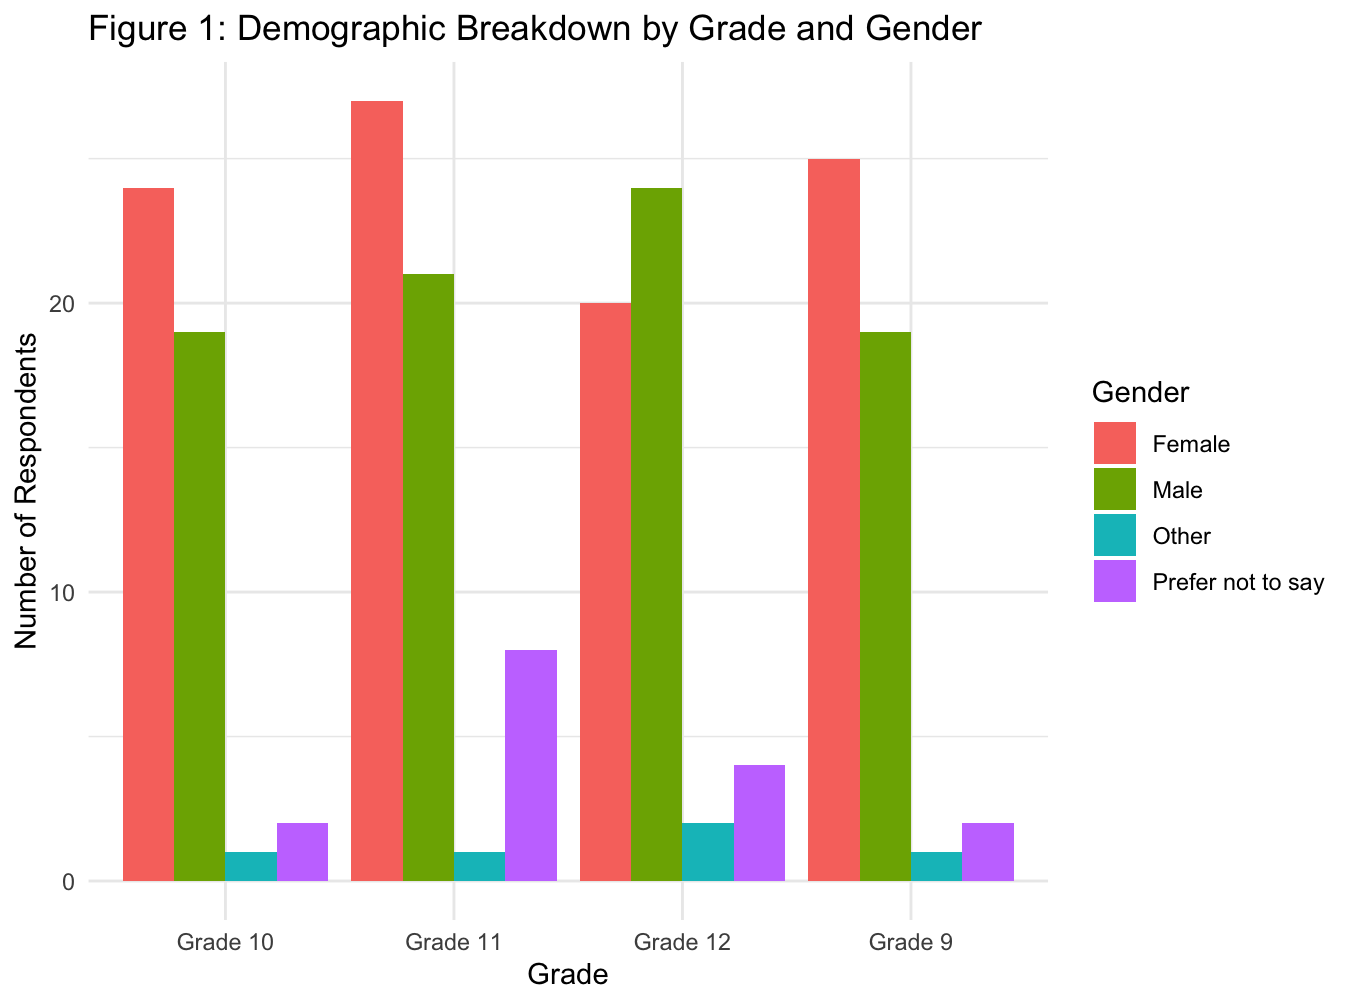
\includegraphics[width=0.85\textwidth,height=\textheight]{plot1.png}\\
The sample was relatively balanced across grades, though Grade 11 showed
slightly higher female participation. Both male and female respondents
were well represented, with smaller but notable counts of students
selecting ``Other'' or ``Prefer not to say.'' This inclusion highlights
gender diversity beyond the binary and ensures voices from all groups
were captured. Overall, the demographic spread supports analysis across
grade levels while acknowledging limitations in sample generalizability.

The main variables of interest are the five \textbf{needs assessment
items}, which asked students to rate the importance of topics such as
course planning, extracurriculars, mental health, scholarship
information, and university admissions. Responses used a 5-point Likert
scale, with higher values indicating greater importance.\\
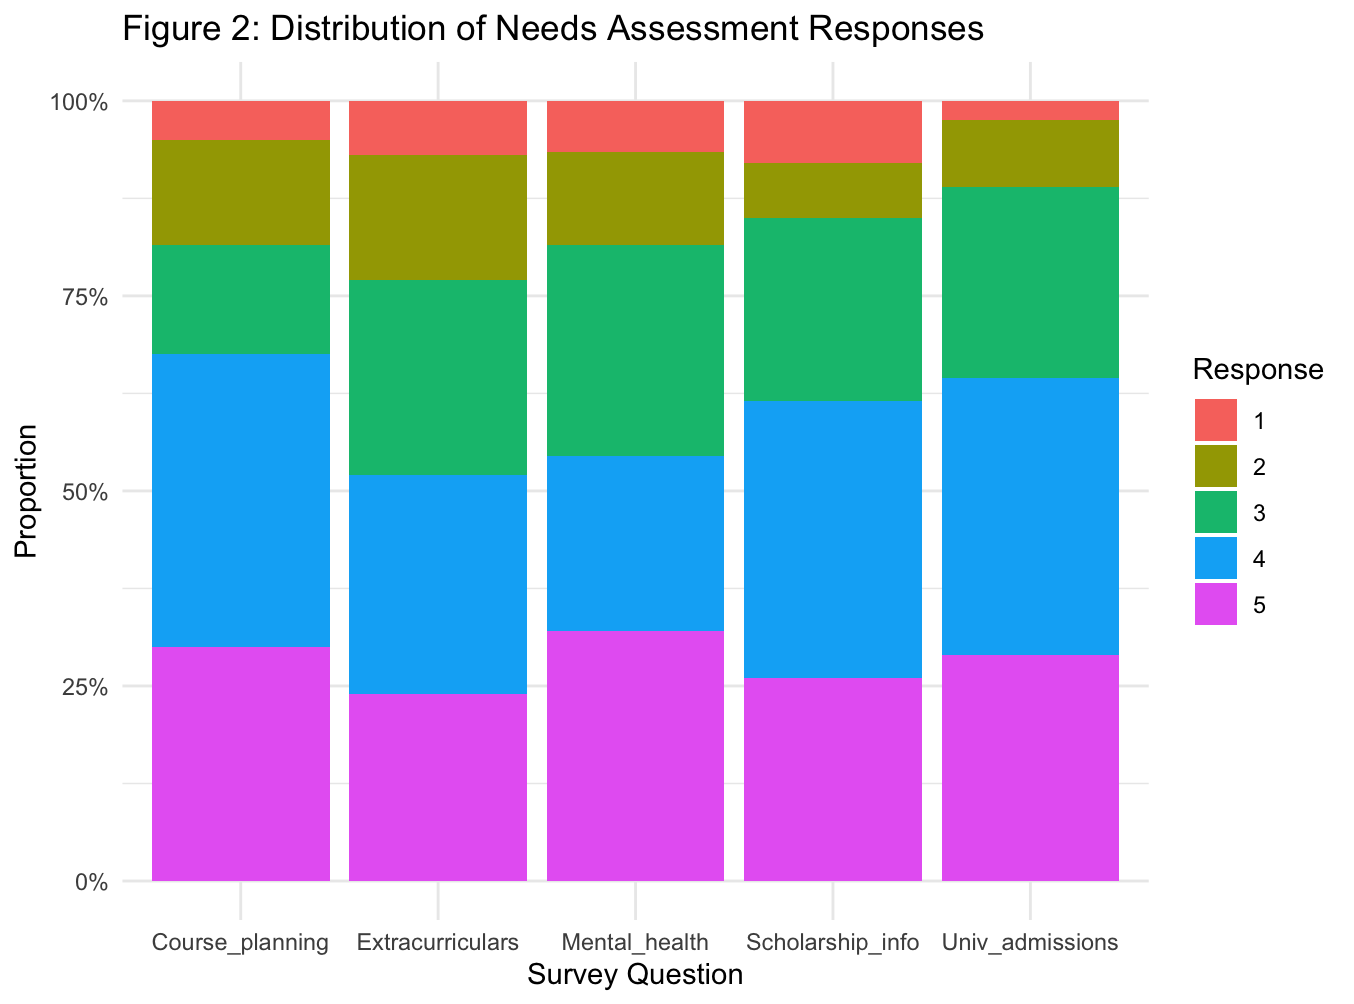
\includegraphics[width=0.85\textwidth,height=\textheight]{plot2.png}\\
Scholarship information, university admissions, and course planning were
most frequently rated as ``very'' or ``extremely'' important (scores
4--5). Mental health and extracurriculars also received strong support
but showed a slightly wider spread of responses, suggesting that while
these areas matter, they may not be equally prioritized by all students.
These patterns align with the survey's purpose: identifying handbook
topics that require emphasis to best support underserved students.

The survey also included a multi-select question on
\textbf{underrepresented group membership}. Students could identify with
one or more categories (e.g., women in STEM, 2SLGBTQ+, new
immigrant/ESL, racial minority, disabled,
low-income/first-generation).\\
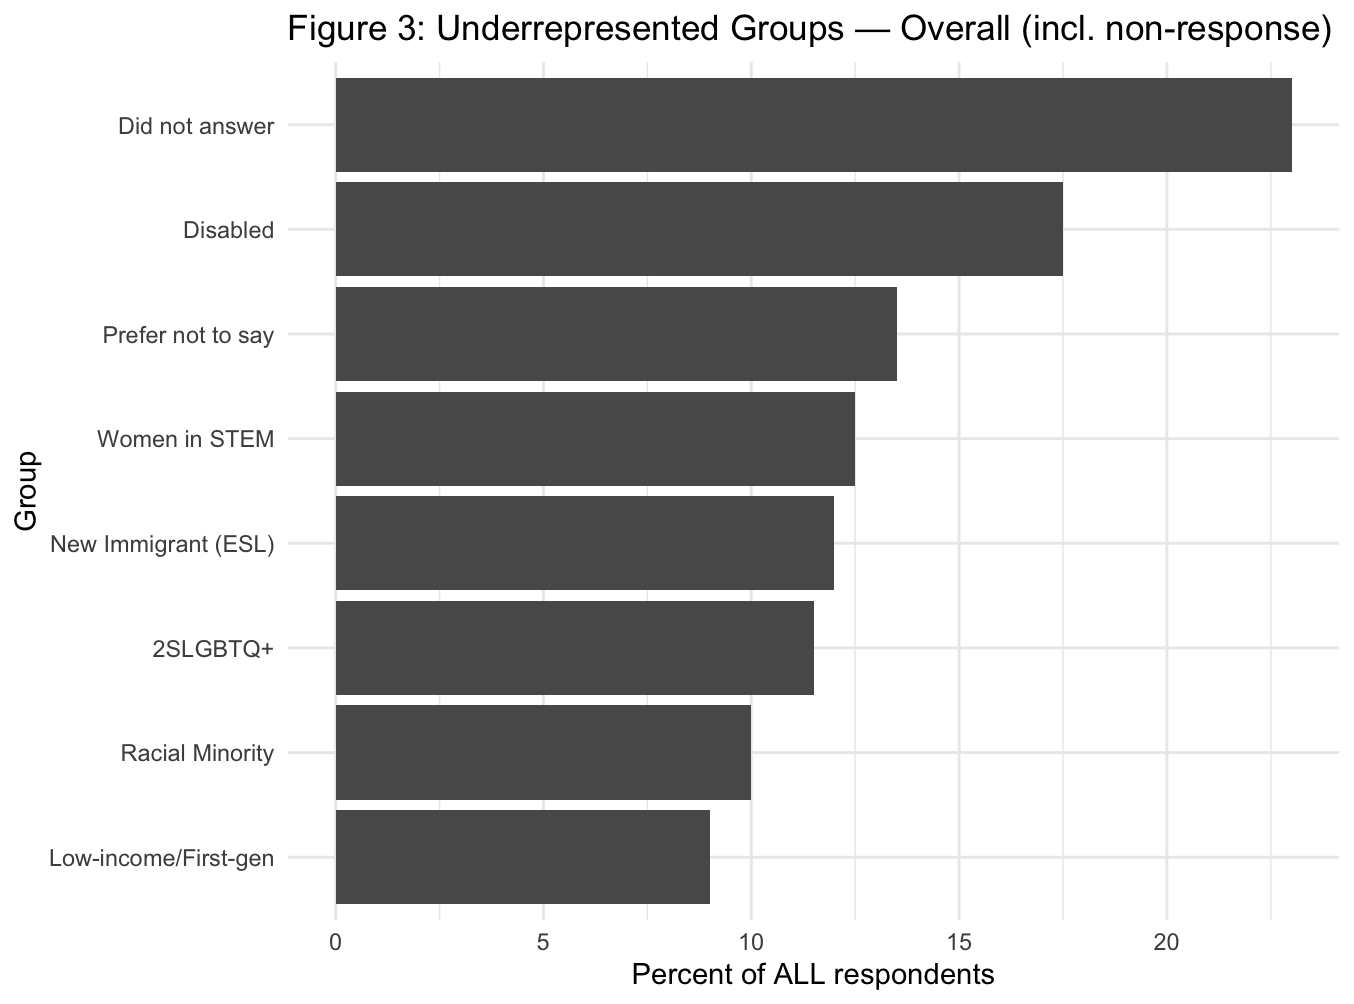
\includegraphics[width=0.85\textwidth,height=\textheight]{plot3.png}\\
Roughly 20\% of students did not provide a response, which may indicate
discomfort with disclosure or survey fatigue. Or simply, that they are
not a part of any underrepresented group mentioned. Among those who
answered, meaningful representation was observed across categories, with
particularly high counts in ``Disabled'' and ``Women in STEM.'' This
provides evidence that STEMBuddies is reaching diverse subgroups, though
the non-response rate should be kept in mind when interpreting these
results.

Finally, the data section sets up our inferential analysis. Later, we
will calculate a confidence interval for one of the needs assessment
variables---for example, the proportion of students rating
\textbf{scholarship information} as ``extremely important.'' From Figure
2, this item appears to have a notably high endorsement rate, making it
both substantively interesting and statistically appropriate for
interval estimation. Establishing a margin of error around this
proportion will help quantify how confident we can be that high
scholarship information demand extends beyond our sample.

\section{Methods}\label{methods}

Our primary inferential analysis focuses on the proportion of students
who rated \emph{scholarship information} as ``extremely important'' in
the needs assessment section of the survey. Because this outcome is
categorical (students either did or did not select the highest rating),
the appropriate statistical tool is a \textbf{confidence interval for a
population proportion}. This allows us to estimate, with a stated level
of confidence, the true proportion of all students who would give this
response if the survey were administered to the broader population.

The general formula for a confidence interval for a proportion is:

\[\[ \hat{p} ; \pm ; z\_{\alpha/2} \cdot \sqrt{\frac{\hat{p}(1-\hat{p})}{n}} \]\]

Here, \[(\hat{p})\] is the sample proportion of students in our dataset
who selected ``extremely important,'' \[(n)\] is the total sample size,
and \[(z\_{\alpha/2})\] is the critical value from the standard normal
distribution corresponding to the chosen confidence level (for a 95\%
confidence interval, \[(z\_{\alpha/2} \approx 1.96))\]. The square root
term is the \textbf{standard error}, which measures how much the sample
proportion is expected to vary due to random sampling.

This approach assumes that the sample size is large enough for the
sampling distribution of \[(\hat{p})\] to be approximately normal, a
condition met here with 200 respondents. Interpreting a 95\% confidence
interval means that, if we repeated the study many times, about 95\% of
the intervals constructed in this way would contain the true population
proportion. This method therefore quantifies the uncertainty around our
estimate of how important scholarship information is to students,
preparing the reader to interpret the numerical results in the next
section.

\section{Results}\label{results}

We estimated the proportion of students who rated \emph{scholarship
information} as ``extremely important'' and constructed a 95\%
confidence interval for this estimate. The results are shown in Table 1.

\textbf{Table 1. Estimated proportion and 95\% confidence interval for
students rating scholarship information as extremely important (n =
200).}

\begin{longtable}[]{@{}llll@{}}
\toprule\noalign{}
Estimate & 95\% CI Lower & 95\% CI Upper & N \\
\midrule\noalign{}
\endhead
\bottomrule\noalign{}
\endlastfoot
0.26 & 0.199 & 0.321 & 200 \\
\end{longtable}

Table 1 indicates that approximately 26\% of surveyed students rated
scholarship information as extremely important. The 95\% confidence
interval ranges from about 20\% to 32\%, suggesting that even when
accounting for sampling variability, only about one-quarter to one-third
of the student population would be expected to prioritize scholarship
information at the highest level.

These findings are consistent with earlier descriptive analyses, which
showed strong but not universal endorsement of financial aid resources.
The interval width is relatively narrow, reflecting the stability of the
estimate with a sample size of 200. This result appears reasonable given
the context: while scholarships are a significant concern for many
students, not all view them as the single most critical element compared
to other academic or well-being needs.

Taken together, these results highlight a clear but selective demand for
scholarship guidance, which directly informs STEMBuddies' efforts to
balance financial, academic, and personal support in its handbook. The
following Discussion section expands on these implications and considers
how they align with the broader mission of supporting underserved
students in STEM.

\subsection{Generative AI / Workflow
Statement}\label{generative-ai-workflow-statement}

For this assignment, I used generative AI tools (specifically ChatGPT)
to support my workflow in several ways:

\begin{itemize}
\tightlist
\item
  \textbf{Coding Support in R:} I used AI to help debug and write
  portions of the R code for simulating survey data (e.g., generating
  Likert-scale responses, handling multi-select variables, and producing
  plots such as histograms and bar charts).\\
\item
  \textbf{Idea Generation:} I consulted AI for brainstorming survey
  questions aligned with the STEMBuddies handbook goals, and for
  formatting possible report structures.
\end{itemize}

To ensure that the final report was my own work, I carefully reviewed
and revised all AI-generated content. I verified citations independently
to confirm their relevance and accuracy, and I rewrote or adjusted text
where needed to align with my own understanding and the assignment
requirements. For R code, I ran and tested the code myself in RStudio,
debugging and modifying until the output matched the expected structure.

In summary, AI tools were used to \emph{supplement} my work---offering
drafting assistance, coding guidance, and brainstorming ideas---but the
final analysis, critical thinking, and interpretations are my own.

\subsection{Bibliography}\label{bibliography}

American Statistical Association. (2016). \emph{Guidelines for survey
research methods}. Alexandria, VA: ASA.~~

Creswell, J. W., \& Creswell, J. D. (2018). \emph{Research design:
Qualitative, quantitative, and mixed methods approaches} (5th ed.).
Thousand Oaks, CA: Sage.~~

Museus, S. D., Palmer, R. T., Davis, R. J., \& Maramba, D. C. (2011).
\emph{Racial and ethnic minority students' success in STEM education}.
ASHE Higher Education Report, 36(6), 1--140.~~

National Academies of Sciences, Engineering, and Medicine. (2016).
\emph{Barriers and opportunities for 2-year and 4-year STEM degrees:
Systemic change to support students' diverse pathways}. Washington, DC:
National Academies Press. https://doi.org/10.17226/21739~~

STEMBuddies. (2025). \emph{STEMBuddies high school handbook}. Retrieved
from https://stembuddies.ca

\section{Appendix}\label{appendix}

\subsection{A. Survey Questions}\label{a.-survey-questions}

\textbf{Introduction Message:}\\
\emph{Thank you for participating in the STEMBuddies High School
Handbook Survey. Your responses will help us improve the handbook so it
better supports students like you in areas such as course planning,
scholarships, admissions, extracurriculars, and mental health. All
responses are anonymous and will only be used for research purposes.}

\begin{center}\rule{0.5\linewidth}{0.5pt}\end{center}

\subsubsection{Section 1: Demographic
Questions}\label{section-1-demographic-questions}

\begin{enumerate}
\def\labelenumi{\arabic{enumi}.}
\tightlist
\item
  \textbf{What grade are you currently in?}

  \begin{itemize}
  \tightlist
  \item
    Grade 9\\
  \item
    Grade 10\\
  \item
    Grade 11\\
  \item
    Grade 12
  \end{itemize}
\item
  \textbf{What is your gender identity?}

  \begin{itemize}
  \tightlist
  \item
    Male\\
  \item
    Female\\
  \item
    Other (please specify)\\
  \item
    Prefer not to say
  \end{itemize}
\item
  \textbf{Do you identify as belonging to one or more of the following
  groups underrepresented in STEM?} (Select all that apply) (optional)

  \begin{itemize}
  \tightlist
  \item
    Women in STEM\\
  \item
    2SLGBTQ+\\
  \item
    New immigrant / ESL\\
  \item
    Racial minority\\
  \item
    Disabled\\
  \item
    Low-income / first-generation student\\
  \item
    Prefer not to say
  \end{itemize}
\end{enumerate}

\begin{center}\rule{0.5\linewidth}{0.5pt}\end{center}

\subsubsection{Section 2: Needs
Assessment}\label{section-2-needs-assessment}

\begin{enumerate}
\def\labelenumi{\arabic{enumi}.}
\setcounter{enumi}{3}
\tightlist
\item
  \textbf{How important is access to information about course planning
  in supporting your academic goals?}

  \begin{itemize}
  \tightlist
  \item
    Not Important\\
  \item
    Slightly Important\\
  \item
    Moderately Important\\
  \item
    Important\\
  \item
    Very Important
  \end{itemize}
\item
  \textbf{How important is access to information about scholarships and
  financial aid in supporting your high school and postsecondary goals?}

  \begin{itemize}
  \tightlist
  \item
    Not Important\\
  \item
    Slightly Important\\
  \item
    Moderately Important\\
  \item
    Important\\
  \item
    Very Important
  \end{itemize}
\item
  \textbf{How important is access to information about university
  admissions requirements and processes?}

  \begin{itemize}
  \tightlist
  \item
    Not Important\\
  \item
    Slightly Important\\
  \item
    Moderately Important\\
  \item
    Important\\
  \item
    Very Important
  \end{itemize}
\item
  \textbf{How important is access to information about extracurricular
  opportunities?}

  \begin{itemize}
  \tightlist
  \item
    Not Important\\
  \item
    Slightly Important\\
  \item
    Moderately Important\\
  \item
    Important\\
  \item
    Very Important
  \end{itemize}
\item
  \textbf{How important is access to resources and information about
  mental health?}

  \begin{itemize}
  \tightlist
  \item
    Not Important\\
  \item
    Slightly Important\\
  \item
    Moderately Important\\
  \item
    Important\\
  \item
    Very Important
  \end{itemize}
\end{enumerate}

\begin{center}\rule{0.5\linewidth}{0.5pt}\end{center}

\textbf{Closing Message:}\\
\emph{Thank you for completing the survey! Your feedback will directly
inform updates to the STEMBuddies High School Handbook. If you'd like to
learn more about our work, please visit our website.}

\begin{center}\rule{0.5\linewidth}{0.5pt}\end{center}

\subsection{B. Glimpse of Simulated
Data}\label{b.-glimpse-of-simulated-data}



\end{document}
